\documentclass{article}

\usepackage[utf8]{inputenc}
\usepackage[T1]{fontenc}      
\usepackage[francais]{babel}
\usepackage{graphicx}
\usepackage{circuitikz}
\usepackage[squaren, Gray]{SIunits}
\usepackage{sistyle}
\usepackage[autolanguage]{numprint}
\usepackage{pgfplots}
\pgfplotsset{compat=1.9}
\usepackage{amsmath,amssymb,array}
\usepackage[top=2.5cm,bottom=2.5cm,right=2.5cm,left=2.5cm]{geometry}
\usepackage{url} 
\usepackage{tabularx}
\DeclareMathOperator{\dist}{d}
\newenvironment{abstract-fr}
{
	\begin{center}
		\textbf{Résumé} \\[0.5cm]
	\end{center}
}
{}

\newenvironment{abstract-en}
{
	\begin{center}
		\textbf{Summary} \\[0.5cm]
	\end{center}
}
{}
% New command pour la modélisation mécanique, tri à effectuer
\newcommand\fv[1]{{\bf #1}} % free vector
\newcommand\fvd[1]{\dot{\bf #1}} % free vector derivated
\newcommand\fvdd[1]{\ddot{\bf #1}} % free vector derivated
\newcommand\fvr[1]{\mathring{\bf #1}} % free vector relatively derivated
\newcommand\fvrr[1]{\overset{\circ\circ}{\bf #1}} % free vector relatively derivated
\newcommand\uv[1]{{\bf\hat{ #1}}} % unit vector
\newcommand\ui{{\bf\hat{I}}} % unit vector I
\newcommand\uj{{\bf\hat{J}}} % unit vector J
\newcommand\uk{{\bf\hat{K}}} % unit vector K
\newcommand\wrt[2]{\ensuremath{\tensor*[_{ #1}]{ #2}{}}} % With Respect To
\newcommand\wtr[3]{\ensuremath{\tensor*[_{ #1}]{ #2}{^{ #3}}}} % With Two Respect
\newcommand\omegaf{{\bm \omega}}
\newcommand\omegafr{\mathring{\bm \omega}}
\newcommand\omegafd{\dot{\bm \omega}}
\newcommand\omegaft{\tilde{\bm \omega}}
\newcommand\omegaftr{\mathring{\tilde{\bm \omega}}}
\newcommand\omegat{\tilde{\omega}}
\newcommand\omegatd{\tilde{\dot{\omega}}}
\newcommand\ine{{\bf I}}
\newcommand\st{{\bf L}}
\newcommand\pst{{\bf M}}
\newcommand\lm{{\bf N}}
\newcommand\am{{\bf H}}
\newcommand\amd{\dot{\am}}
\newcommand\fo{{\bf F}}
\newcommand\po{\mathcal{P}}
\newcommand\xg{\ensuremath{\fv{R}}}
\newcommand\xgd{\ensuremath{\fvd{R}}}
\newcommand\xgdd{\ensuremath{\fvdd{R}}}
\newcommand\dvec[1]{\dot{\vec{ #1}}}
\newcommand\ddvec[1]{\ddot{\vec{ #1}}}
\newcommand\qp{\dot{q}}
\newcommand\dqp{\Delta \dot{q}}
\usepackage{url} 
\usepackage{hyperref}
\hypersetup{
    colorlinks,
    citecolor=black,
    filecolor=black,
    linkcolor=black,
    urlcolor=black
}

\begin{document}

\section{Modélisation mécanique du haut-parleur}

\subsection{Composition du haut-parleur}
Le haut-parleur est constitué de différentes parties : une membrane
attachée par des fixations qui jouent le rôle de ressorts et reliée à 
une bobine mobile et une bobine fixe qui s'emboîte (sans frottement) 
dans cette dernière.

La bobine fixe va permettre à la bobine mobile de se déplacer exclusivement de gauche
à droite (voir Figure \ref{hp-scheme}), permettant ainsi à la membrane de vibrer 
(et donc de produire un son). Tout déplacement dans une autre direction serait dommageable
car risquerait d'abîmer la membrane.

\begin{figure}[ht!]
	\centering
	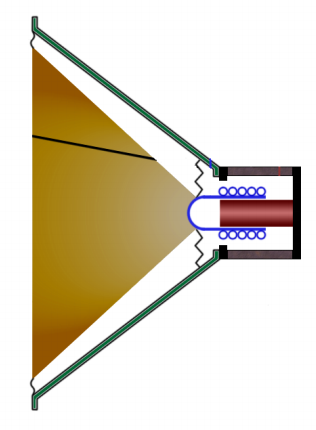
\includegraphics[scale=0.6]{haut-parleur.png}
	\caption{Schéma d'un haut-parleur. (Source : \textit{Modélisation mécanique du haut-parleur} sur iCampus)}
	\label{hp-scheme}
\end{figure}

\subsection{Étude du mouvement de la bobine mobile}
Nous allons maintenant écrire les équations du mouvement de la bobine mobile.
Pour ce faire, nous plaçons un repère fixe $\{\ui\}$ dont l'origine $O$ se trouve
au centre de gravité de la bobine mobile à sa position d'équilibre (au 
temps $t=0$). $\uv{I}_1$ est parallèle à la bobine et dirigé vers la gauche, tandis que
$\uv{I}_2$ est dirigée perpendiculairement à la bobine mobile, vers le haut.
La bobine mobile ne possède qu'un seul degré de liberté, qui
est la distance entre $O$ et son centre de gravité; notons-la $\fv{x}(t)$.
La positon de la bobine est donc donnée par :

$$\vec{R(t)} = \fv{x}(t) \uv{I}_1$$ 

\paragraph{Inventaire des forces}
Avant d'écrire l'équation du mouvement de la bobine, établissons l'inventaire
des forces qui agissent sur celle-ci :

\begin{itemize}
	\item Son poids, dont la résultante agit sur son centre de gravité : $-mg\uv{I}_2$ ;
	\item La force de rappel des fixations (que l'on suppose agir comme des simples
	ressorts) : $-k \fv{x}(t) \uv{I}_1$ où $k$ est la constante de raideur des fixations ;
	\item La force électromagnétique causée par l'électroaimant : $BLi(t) \uv{I}_1$ où
	$B$ est le champ magnétique produit par l'électroaimant, $L$ la longueur de fil de cuivre
	utilisé et $i(t)$ le courant électrique ;
	\item Le frottement dû à l'air ;
\end{itemize}

Parmis toute ces forces, nous négligeons le frottement dû à l'air ainsi que le poids
de la bobine mobile (sa masse étant relativement faible).

\paragraph{Équation du mouvement}
Nous avons maintenant tout à notre disposition pour écrire les équations du mouvement
\footnote{Dans cette section, nous utilisons les notations employées au cours de
mécanique des corps rigides.} :

$$m\fvdd{x}(t) = -k\fv{x}(t) + BLi(t)$$

En sachant que le signal d'entrée est une fonction de la forme $V(t) = V_0 \cos (\omega t)$ et
que, par la loi d'Ohm, $V(t) = Ri(t)$ où $R$ est la résistance du circuit, 
nous pouvons réecrire l'équation différentielle du mouvement de la manière suivante :

$$m\fvdd{x}(t) + k\fv{x}(t) = \frac{B2\pi rNV_0}{R}\cos (\omega t)$$

Où nous avons également fait apparaître le nombre de spires $N$ et le rayon de la bobine
$r$. Il ne reste donc plus qu'à résoudre cette équation différentielle.

\paragraph{Résolution de l'équation différentielle du mouvement}
Résolvons cette équation différentielle comme appris lors de ce deuxième
quadrimestre. Cherchons d'abord la solution homogène de cette équation, notée $\fv{x}_h(t)$.
Pour ce faire, résolvons le polynôme caractéristique :

$$mr^2 + k = 0 \Rightarrow r = \pm i\sqrt{\frac{k}{m}}$$

Nous avons donc, en ne gardant que la partie réelle :

$$\fv{x}_h(t) = Ae^{i\sqrt{\frac{k}{m}}t} + Be^{-i\sqrt{\frac{k}{m}}}$$

Où $A$ et $B$ sont des coéfficients complexes. Nous pouvons réecrire cette solution
en termes de fonctions trigonométriques. En ne gardant que la partie réelle, 
nous obtenons :

$$\fv{x}_h(t) = C\cos(\sqrt{\frac{k}{m}}t) - D\sin(\sqrt{\frac{k}{m}}t)$$

Où $C$ et $D$ sont cette-fois des coefficients réels.

Penchons-nous maintenant sur la solution particulière, notée $\fv{x}_p(t)$. Pour
cette partie de la résolution, nous réécrivons le terme non-homogène sous la forme d'une
exponentielle complexe. La solution particulière est de la forme :

$$\fv{x}_p(t) = \alpha e^{\omega it}}$$

En injectant $\fv{x}_p(t)$ et sa dérivée seconde dans l'équation de départ, nous trouvons :

$$\alpha = \frac{2\pi rNV_0}{R(-m\omega^2 + k)} \Rightarrow \fv{x}_p(t) = \frac{2\pi rNV_0}{R(-m\omega^2 + k)}e^{wit}$$

En ne gardant que la partie réelle de l'exponentielle, nous avons finalement :

$$\fv{x}_p(t) = \frac{2\pi rNV_0}{R(-m\omega^2 + k)} \cos (\omega t)$$

Par le principe de superposition des solutions des équations différentielles :

$$\fv{x}(t) = \fv{x}_h(t) + \fv{x}_p(t) = C\cos(\sqrt{\frac{k}{m}}t) - D\sin(\sqrt{\frac{k}{m}}t) + \frac{2\pi rNV_0}{R(-m\omega^2 + k)} \cos (\omega t)$$

En utilisant la première condition initiale, $\fv{x}(0) = 0$, nous trouvons:

$$C = \frac{-BLV_0}{R(-m\omega^2+k}$$

Il reste à trouver une deuxième condition initiale.

\subsection{Fréquence de résonance}
Nous remarquons que si $\omega \rightarrow \sqrt{\frac{k}{m}}$, le dénominateur de l'amplitude du mouvement
tend vers \numprint{0}, et donc l'amplitude du mouvement tend vers $\infty$. Cette situation n'a physiquement
pas de sens. Nous notons cette fréquence $\omega_0$; il s'agit de la \textit{fréquence de résonance}.

\subsection{Couplage entre mouvement et son émis}
Étudions maintenant le mouvement de la deuxième couche
d'air representée sur la Figure \ref{wave-sound-scheme}.
La couche numérotée \numprint{0} représente la membrane.
La pression dans la couche d'air numérotée \numprint{1} 
est $p_0 + dp(t)$. Dans les couches suivantes, elle est
constante vaut $P_0$. Nous considérons un problème simplifié
à une dimension (déplacement de tranche d'air dans un
tuyau). Nous prenons également l'hypothèse que les couches
d'air sont incompressibles afin de pouvoir appliquer
ce que nous avons appris au cours de mécanique des corps
rigides.

Plaçons le repère inertiel ${\ui}$ tel que $\uv{I}_1$
est orienté vers la droite horizontalement et $\uv{I}_2$
orienté vers le haut verticalement. Plaçons l'origine
$O$ de ce repère à la position initiale de la couche
d'air. La position de la couche d'air, notée $\vec{R(t)}$ vaut 
donc :

$$\vec{R(t)} = \fv{x}(t)\uv{I}_1$$

\begin{figure}[ht!]
	\centering
	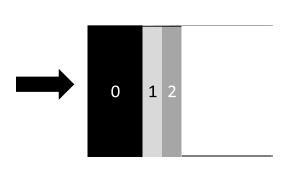
\includegraphics[scale=0.85]{sound-waves.png}
	\caption{Déplacement de tranche de couche d'air dans un tuyau. (Source : \textit{Modélisation mécanique du haut-parleur} sur iCampus)}
	\label{wave-sound-scheme}
\end{figure}

\paragraph{Inventaire des forces}
Comme pour la bobine mobile, faisons l'inventaire
des forces qui s'exercent sur la deuxième couche d'air :

\begin{itemize}
	\item Le poids de la couche d'air : $-\rho A\uv{I}_2$, ou $\rho$ est la densité volumique
	de l'air et $A$ est la surface de la couche d'air ;
	\item La pression exercée sur la couche \numprint{2} par la pression dans la couche \numprint{1}
	: $(p_0 + dp(t))A \uv{I}_1$.
\end{itemize}

\paragraph{Équation du mouvement}
Nous pouvons maintenant écrire l'équation du mouvement

% Just here to fix rapport_prejury.tex
\end{document}
